%%%%%%%%%%%%%%%%%%%%
%  DOCUMENT CLASS  %
%%%%%%%%%%%%%%%%%%%%

\documentclass[hyphens,twocolumn,nobalancelastpage,aps,10pt,citeautoscript,longbibliography]{revtex4-2}

%%%%%%%%%%%%%%
%  PACKAGES  %
%%%%%%%%%%%%%%
\nonstopmode%
\usepackage{url}
\usepackage[table,xcdraw,svgnames]{xcolor}
\usepackage{listings,engord,graphicx,bm,xfrac,newpxtext,physics,siunitx}
\AtBeginDocument{\RenewCommandCopy\qty\SI}
\usepackage{natbib}
\usepackage[colorlinks]{hyperref}
\hypersetup{
	colorlinks=true,
	citecolor=black,
	linkcolor=DimGrey,
	urlcolor=DimGrey,
	breaklinks=true
}
\usepackage[english]{babel}
\usepackage[T1]{fontenc}
\usepackage[version=4]{mhchem}
\usepackage[a4paper, portrait, margin=2.54cm]{geometry}
\usepackage[compact]{titlesec}
\usepackage{color}
\definecolor{deepblue}{rgb}{0,0,0.5}
\definecolor{deepred}{rgb}{0.6,0,0}
\definecolor{deepgreen}{rgb}{0,0.5,0}

%%%%%%%%%%%%%%
%  SETTINGS  %
%%%%%%%%%%%%%%

% \graphicspath{ {./images/} }

\setlength{\parskip}{1em} \lstdefinestyle{mystyle}{
	commentstyle=\color{deepgreen}, keywordstyle=\color{deepred},
	stringstyle=\color{codeblue}, basicstyle=\ttfamily,
	breakatwhitespace=false, breaklines=true,
	emphstyle=\ttb\color{deepred}, captionpos=b, keepspaces=true,
	numbers=left, numbersep=5pt, showspaces=false,
	showstringspaces=false, showtabs=false, tabsize=2 }
\lstset{style=mystyle}

\newcommand{\cay}[1]{\citeauthor{#1} (\citeyear{#1})~\cite{#1}}
\newcommand{\rhob}[0]{\rho_\textrm{bulk}}
\newcommand{\density}[0]{\kilogram\per\metre\cubed}

%%%%%%%%%%%%%%%%%%%%%%
%  DOCUMENT CONTENT  %
%%%%%%%%%%%%%%%%%%%%%%

\begin{document}

\title{Technical report: Exercise 4}

\author{N. Pham}

\begin{abstract}
	For Problem 1, one-body gravitational scenario was modelled with success,
	escape velocity at surface was found to be \qty{11500}{\metre\per\second}.
	Principle of energy conservation was observed to hold, and a step size at
	around \qty{e1}{\second} was deemed adequate for the one-body model.
	Initial parameters were found for a rocket to perform a round trip between
	earth and moon, drawing a ``figure 8'' shape.

	For Problem 2, two-body interactions have been modelled, with worse
	accuracy than the one-body interaction at high kinetic energies or close
	proximity scenarios. Stable orbits for earth-moon and earth-moon-sun
	systems were achieved using mean physical values for speed and separation.
	However, moon eccentricity (found to be $\sim$0.42), or and the number of
	sidereal month (found to be 13.5 months) in a year was not accurate, due to
	a combination of the nature of numerical solvers and other physical factors
	not taken into account.
\end{abstract}

\maketitle

\section{PROBLEM 1: ROCKET ORBITS}%
\label{sec:problem_1}

\subsection{Introduction}%
\label{sub:introduction_1}

\noindent Problem 1 required using the Runge-Kutta method to model the motion
of a rocket under t he influence of the earth's and/or moon's gravitational
field.

Part (a) asked to model a rocket moving in earth's gravitational field. Part
(b) asked to model a rocket moving in earth's and moon's gravitational fields,
and find the set(s) of initial conditions where the rocket starts from low
earth orbit, passes over the moon's, and using its gravitational field
(slingshot) to return to earth without crashing into either body.

\subsection{Theory}%
\label{sub:theory_1}

\noindent The Runge-Kutta method is a numerical method. For a two-dimensional
system with 4 dependent variables $x$, $y$, $v_x$ and $v_y$---from now on written with the format ($x, y, v_x, v_y$)---with a step-size $h$, the
system variables at timestep $t_i$ are:

\begin{equation}
	\label{eq:timestepping}%
	\begin{split}
		a_{i+1}   & = a_i + \frac{h}{6}\left[k_{1a}+2k_{2a}+2k_{3a}+k_{4a}\right] \\
		t_{i+1} &= t_i + h
	\end{split}
\end{equation}
where $a$ is the dependent system variable to be calculated. As seen, at each
timestep, 16 $k$'s must be calculated, 4 for each dependent variables, using
the first and second derivatives of the moving body's position vector. The
$k_4$'s depend on the $k_3$'s ($a_i + hk_{3}$), which depend on the $k_2$'s ($a_i +
	hk_{2}/2$), which depend on the $k_1$'s ($a_i + hk_{1}/2$)

The values of $k_{n,a}$ for $n$ from 1 to 4 depends on $a$, where

\begin{equation}
	\label{eq:k_equations}%
	\begin{split}
		k_{n,x} &= \dot{x}\\
		k_{n,y} &= \dot{x}\\
		k_{n,v_{x}} &= \ddot{x}\\
		k_{n,v_{y}} &= \ddot{y}
	\end{split}
\end{equation}

The equation of motion for part (a) gives

\begin{equation}
	\label{eq:part_a}%
	\ddot{\mathbf{r}} = - \frac{M_EG\mathbf{r}}{{\left|\mathbf{r}\right|}^3}
\end{equation}
where $M_E$ is the mass of the earth, $m$ is the mass of the rocket, $G$ is the
gravitational constant, and $\mathbf{r}$ is the position vector of the rocket
with the centre of earth as the origin.

The equation of motion for part (b) gives

\begin{equation}
	\label{eq:part_b}%
	\ddot{\mathbf{r}} = - G\left(\frac{M_E\left(\mathbf{r} - \mathbf{R_E}\right)}{{\left|\mathbf{r} - \mathbf{R_E}\right|}^3} + \frac{M_M\left(\mathbf{r} - \mathbf{R_M}\right)}{{\left|\mathbf{r} - \mathbf{R_M}\right|}^3}\right)
\end{equation}
where $M_M$ is the mass of the moon, and $\mathbf{R_E}$ and $\mathbf{R_M}$ are
the position vectors of the earth and the moon respectively. Placing the Earth
at the origin sets $\mathbf{R_E = 0}$.

\subsection{Method}%
\label{sub:method_1}

\noindent For part (a), the earth was set at the origin and the rocket's
initial conditions are requested as user inputs, as well as the maximum time
\lstinline{max_time} to render the simulation (giving
\lstinline{max_time}/$h$-sized arrays). The Runge-Kutta, written manually,
calculates and returns the positions and velocities of the rocket at all
timesteps as 4 different arrays, one for each dependent variable. The timestep
was hard-coded to $h=\qty{40}{\second}$.

The potential and kinetic energy at each timestep was also calculated, as well
as the total energy (the sum of potential and kinetic energy). From
conservation of energy, the total energy of a system must be conserved. Since
the total energy at each timestep is individual and independent, the standard
deviation in total energy can be calculated. Finally, the relationship between
step size $h$ and the standard deviation in total energy is investigated with
rocket's initial conditions set to ($\qty{0}{\metre}, 1.1 R_E,
	\qty{-10000}{\metre\per\second}, \qty{0}{\metre\per\second}$) and modelled for
\qty{30000}{\second}. Values of $h$ ranged from \qty{10}{\second} to
\qty{200}{\second}, with 400 values of $h$ in total.

To determine the status of the trajectory (i.e.\ the rocket has not crashed),
the distance between rocket (a point source) and the earth has to remain less
than $R_E$.

For part (b), the same Runge-Kutta method was used as in part (a), but changing
the equations that populate the values of $k$'s to correspond to
Eq.~\ref{eq:part_b}. The earth remains at the origin and the moon introduced at
coordinate $(0,\qty{3.84e8}{\metre})$. User inputs the same parameters as part (a). The rocket
has to undergo an extra check to check whether it has crashed into the moon.
The initial conditions where the rocket does a round trip without crashing was
found with trial and error.

\subsection{Results \& discussions}%
\label{sub:results_and_discussions_1}

\noindent For part (a), several different trajectories can be simulated using
this one body algorithm (see Fig.~\ref{fig:./assets/part_a}). If the trajectory
is an orbit, it is an ellipse. An ellipse is characterised by its major and
minor axes, and if these two quantities are the same, then the orbit is
circular. The program is able to calculate this ratio, a value which is only
valid for orbits and not trajectories which end in a crash.

\begin{figure*}[htpb]
	\centering
	\includegraphics[width=\linewidth]{./assets/part_a.png}
	\caption{(A): Rocket starting from surfacing and crashing. (B) Near
	circular orbit at surface (before crashing). (C) Elliptical circular orbit
	at surface. (D) Stable low earth orbit. Distance is scaled by $R_E$.}%
	\label{fig:./assets/part_a}
\end{figure*}

The escape velocity at earth surface was also tested. A rocket was launched
$(\qty{0}{\metre}, -R_E)$, and at various y velocities in the negative y
direction. Each simulation was set to run with \lstinline{max_time} $> 1000000$
to ensure rockets near escape velocity have enough time to decelerate to a
halt, and then free fall back to earth. The escape velocity was found to be
\qty{-11500}{\metre\per\second}. A known value of escape velocity at earth's
surface is \qty{11186}{\metre\per\second}~\cite{ev}. The simulation was able to
replicate a value within the same order of magnitude with a very simplistic
model (only earth's gravitational field). In reality, we expect the escape
velocity to also be affected by the distribution of earth's mass, which is not
entirely symmetric.

Fig.~\ref{fig:./assets/total_energy} shows the kinetic and potential energy, as
well as their addition---the total energy. For the scenario modelled and step
size chosen, the total energy stays approximately constant throughout. To
investigate the correlation between step size and error further, rockets were
sent with the same initial conditions 400 times, but at increasing step size
every time. The result is seen in Fig~\ref{fig:./assets/step_size_std_energy}.
The relationship between step size and error is nearly a quartic increase
($\sim 4.27$), with higher step size giving worse accuracy. The error was
deemed negligible at $\sim \qty{e-3}{\joule\per\kilogram}$ order of magnitude,
which gives ideal step sizes in the $\sim\qty{e1}{s}$ order of magnitude. For
the rest of the exercise, the step size was set to $h = \qty{40}{\second}$.

\begin{figure*}[htpb]
	\centering
	\includegraphics[width=\linewidth]{./assets/total_energy.png}
	\caption{Kinetic, potential and total energy of rocket in orbiting earth.}
	\label{fig:./assets/total_energy}
\end{figure*}

\begin{figure*}[htpb]
	\centering
	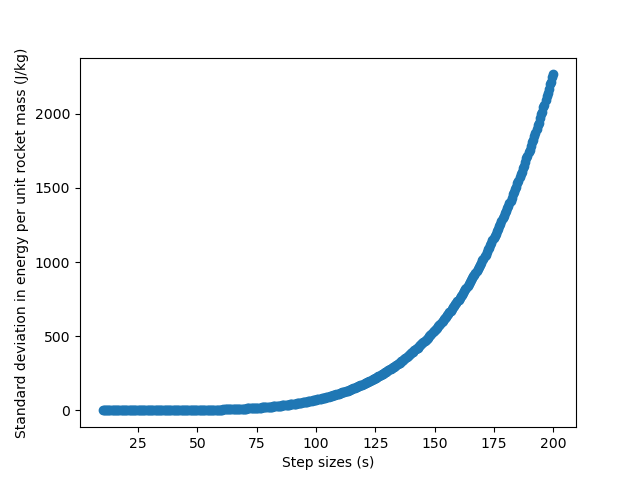
\includegraphics[width=\linewidth]{./assets/step_size_std_energy.png}
	\caption{Left: standard deviation in total energy with respect to step
	size. Right: log plot of standard deviation in total energy with respect to
	step size.}%
	\label{fig:./assets/step_size_std_energy}
\end{figure*}

For part (b), the moon was placed on the vertical as discussed in
Section~\ref{sub:method_1}, and optimum initial conditions for the rocket at
low earth orbit were found to be $(0, -1.09 R_E,
\qty{-10591}{\metre\per\second}, \qty{0}{\metre\per\second})$. It was most
optimal to launch the rocket on the same vertical as the moon's position
vector, but placed on the other side of the earth (see
Fig.~\ref{fig:./assets/figure8}). This allows the rocket to use earth's
gravitational field to curve its trajectory towards the moon, escape earth's
gravitational field, approach moon at a speed just low enough so that it gets
slingshots around the moon and back to earth. The shape of flight is a ``figure
8'' shape, and the orbit shape is roughly maintained as the moon follows almost
same trajectory with consecutive orbits (the snapshot from
Fig.~\ref{fig:./assets/figure8} shows the trajectory of roughly 1.25 orbits).
The round trip was calculated to have taken 9.614 days. It was also found that
the closet approach to the moon, at \qty{6.75e6}{m} from the moon's centre,
which is 2.8 moon radii away from crashing into the moon.

Unlike in part (a), where there was no moon's gravitational field, the
trajectory shape is normally not conserved other than at the optimal initial
conditions stated above. In the right side of Fig.~\ref{fig:./assets/figure8},
the rocket goes to the moon and back twice at the snapshot shown and does not
crash, yet its trajectories are slightly different each time it comes around.

\begin{figure*}[htpb]
	\centering
	\includegraphics[width=\linewidth]{./assets/figure8.png}
	\caption{Left: ``Figure 8'' trajectory of rocket. Rocket begins in
	low-earth orbit, does a loop around the moon, and come back to earth before
	repeating the trajectory. Right: Rocket going past the moon and getting
	slingshot back and around earth, with consecutive orbits unpredictable.
	Distance is scaled by $R_E$.}%
	\label{fig:./assets/figure8}
\end{figure*}

For the initial conditions stated above, the rocket's distance from earth's and
moon's centre were plotted in Fig.~\ref{fig:./assets/figure8_distances}. When
the rocket nears the moon, the distance's slope (the velocity) seems to
decrease slightly before increasing and reaching a sharper peak. This occurs as
the rocket does a closed loop around the moon, and its speed is dramatically
increased by its slingshot around the moon. The time where the rocket is
furthest way from earth occurs before the time where the rocket is closest to
earth. This could mean the trajectory is not exactly symmetrical, so its
closest approach is not at $x=0$ but slightly after it passes $x=0$ into
negative $x$ values.

\begin{figure*}[htpb]
	\centering
	\includegraphics[width=\linewidth]{./assets/figure8_distances.png}
	\caption{Rocket's distance from earth's centre (blue) and from moon's centre (olive) with respect to time.}%
	\label{fig:./assets/figure8_distances}
\end{figure*}

Fig.~\ref{fig:./assets/figure8_energies} shows the kinetic, potential, and
total energy of the ``figure 8'' trajectory. The total energy is seen to be
constant throughout, with spikes in kinetic energy near bodies. At the start,
the rocket was moving fast before it slows down due to earth's gravitational
field pulling it in the negative direction of its motion. In the middle of the
flight, there is a tiny ``hump'' in kinetic energy, indicating its slingshot
around the moon. Finally, when it gets nearer to earth again, its kinetic
energy increases as it is attracted towards earth.

\begin{figure*}[htpb]
	\centering
	\includegraphics[width=\linewidth]{./assets/figure8_energies.png}
	\caption{Kinetic, potential and total energy of rocket in ``figure 8''
	trajectory around earth and moon.}
	\label{fig:./assets/figure8_energies}
\end{figure*}

This is not an accurate physical model, as in 9 days, the moon would have moved
from its original position by an appreciable amount. To improve upon this, one
would require a two body simulation where the earth is fixed and the moon and
rocket moves together with moon and earth's gravitational fields taken into
account.

\subsection{Conclusion}%
\label{sub:conclusion_1}

\noindent In conclusion, one-body gravitational scenario was modelled with
success as known value for escape velocity was found to be close. The
correlation between step size $h$ and model accuracy was investigated using the
principle of energy conservation, and found a step size at around
\qty{e1}{\second} to be adequate for the one-body model. Finally, initial
parameters were found to send a rocket to the moon and back, taken into account
both earth's and moon's gravity. Energy conservation was also observed to apply
in this scenario, and the changes in speed or kinetic energy with respect to
where the rocket is between moon and earth appears to be physically plausible.

\section{PROBLEM 2: EARTH, MOON \& SUN}%
\label{sec:problem_2_wave_equation}

\subsection{Introduction}%
\label{sub:introduction_2}

\noindent Problem 2 required simulating two bodies moving under their combined
gravitational fields using the Runge-Kutta method, implemented previously in
Problem 1.

Part (c) asked to simulate two-body motion, for two bodies with equal radius
and mass, as well as for the earth and the moon. Part (d) asked to simulate
two-body motion for the earth and the moon, but with the sun fixed at the
origin, and the combined gravitational fields include earth's, moon's and
sun's.

\subsection{Theory}%
\label{sub:theory_2}

\noindent The equations of motion for part (c) gives

\begin{equation}
	\label{eq:part_c}%
	\begin{split}
		\ddot{\mathbf{r_1}} &= -\frac{M_2G\left(\mathbf{r_1} - \mathbf{r_2}\right)}{{\left|\mathbf{r_1} - \mathbf{r_2}\right|}^3} \\
		\ddot{\mathbf{r_2}} &= -\frac{M_1G\left(\mathbf{r_2} - \mathbf{r_1}\right)}{{\left|\mathbf{r_2} - \mathbf{r_1}\right|}^3} \\
	\end{split}
\end{equation}
where $\mathbf{r_1}$ and $\mathbf{r_2}$ are position vectors of the first and
second body, respectively, and $M_1$ and $M_2$ are the masses of the first and
second body, respectively.

The equations of motion for part (d) gives

\begin{equation}
    \label{eq:part_d}%
    \begin{split}
        \ddot{r_E} &= -G\left(\frac{M_M\left(\mathbf{r_E} - \mathbf{r_M}\right)}{{\left(\mathbf{r_E} - \mathbf{r_M}\right)}^3} + \frac{M_S\left(\mathbf{r_E} - \mathbf{r_S}\right)}{{\left(\mathbf{r_E} - \mathbf{r_S}\right)}^3}\right)\\
        \ddot{r_M} &= -G\left(\frac{M_E\left(\mathbf{r_M} - \mathbf{r_E}\right)}{{\left(\mathbf{r_M} - \mathbf{r_M}\right)}^3} + \frac{M_S\left(\mathbf{r_M} - \mathbf{r_S}\right)}{{\left(\mathbf{r_M} - \mathbf{r_S}\right)}^3}\right)
    \end{split}
\end{equation}
where $\mathbf{r_S}$ is the position vector of the sun, which can be set to
$\mathbf{0}$ to simplify the equations.

\subsection{Method}%
\label{sub:method_2}

\noindent For part (c), the two bodies' initial conditions are set by user
inputs, whereas before earth was hard-coded to be the origin. The same
Runge-Kutta method was used as in part (a) and (b), but changing the equations
that populate the values of $k$'s to correspond to Eq.~\ref{eq:part_c}. To
model moon's orbit around earth, the earth stays fixed and the moon has a
tangent velocity matching the average physical value of its tangent velocity
around the earth, which was set to $\bar{v}_M = \qty{1000}{\metre\per\second}$.

For part (d), the sun is fixed at the origin and the moon and earth were
initialised using physical values, where the earth travels at $\bar{v}_E =
\qty{2.98e4}{\metre\per\second}$, relative to the sun, and the moon travels at
$\bar{v}_E + \bar{v}_M$ relative to the sun. In this part, the user only inputs
the maximum time to render.

\subsection{Results \& discussions}%
\label{sub:results_and_discussions_2}

\noindent For part (c), simulations of identical bodies are shown in
Fig.~\ref{fig:./assets/part_c_1}, and simulations of earth and moon are shown
in Fig.~\ref{fig:./assets/part_c_2}. With two identical bodies, symmetry is
expected to be seen, as two bodies with equal mass will each experience the
same combined force. This symmetry can be seen in all figures of
Fig.~\ref{fig:./assets/part_c_1}.

\begin{figure*}[htpb]
	\centering
	\includegraphics[width=\linewidth]{./assets/part_c_1.png}
	\caption{(A): Two bodies colliding. (B): Two bodies orbiting each other.
	(C) like (B), but faster, it can be seen they are getting further and
	further apart. (D) Two bodies approaching and deflecting each other's
	otherwise straight path. Distance is scaled by $R_E$.}%
	\label{fig:./assets/part_c_1}
\end{figure*}

For simulations of moon and earth, the earth is fixed at the origin and starts
out stationary.initial conditions of the moon were chosen to match the average
behaviour of the moon's orbit---$(\qty{0}{\metre}, )$. The result is
Fig.~\ref{fig:./assets/part_c_2} (D) (although the moon is moving clockwise
here). The earth's position at the origin is perturbed and shifts to the right
following a trajectory which looks like sequences of half-circles. This is
expected because the moon begins to orbit the earth from the right of the
figure as it's moving clockwise, the earth also moves overall to the right,
towards a common centre of mass of both bodies. When the moon reaches the left
side of the figure, the earth has a velocity in the right direction, so this
only decelerates the earth's motion. The moon then completes one orbit, and the
earth's trajectory would look like a half-circle. Consequently, multiple orbits
lead to multiple half-circles.

In Fig.~\ref{fig:./assets/part_c_2} (A), (B), and (C), the earth does not move
substantially because the moon is moving towards and away from earth at a speed
fast enough to not perturb the position of the earth, as the common centre of
mass of both bodies is nearer to earth if the two bodies are close enough.

\begin{figure*}[htpb]
	\centering
	\includegraphics[width=\linewidth]{./assets/part_c_2.png}
	\caption{(A): Moon plummeting towards the earth. (B): Moon approaching
	earth with sufficient energy to slingshot and escape. (C): Moon deflected
	by earth. (D): Moon orbiting earth and earth's movement due to moon's
	gravitational field. Distance is scaled by $R_E$.}%
	\label{fig:./assets/part_c_2}
\end{figure*}

Conservation of energy was not observed for two equal bodies moving in close
proximity. Fig.~\ref{fig:./assets/two_equal_time_10000000_h_10} represents the
simulation seen in Fig.~\ref{fig:./assets/part_c_1} (B), but for an extended
time to observe the overall total energy, as well as timestep of $h =
\qty{10}{\second}$. The total energy increases logarithmically, with a standard
deviation normally being 3 orders of magnitude lower than the mean energy,
which does not correspond with the findings from
Fig.~\ref{fig:./assets/step_size_std_energy}. This mean that the standard
deviation is not fixed and depends on the scale of the problem. While this
increase is small for bodies far away with less energetic movements---for
bodies close together, their orbits are more violent and thus the total energy
is very sensitive to big values of energ. It shows the Runge-Kutta method
exhibits energy conservation violation in sensitive scenarios such as t his.
The imperfect numerical nature of the method means for complicated models such
as the near-proximity two-body problem, one would have to find a better way to
optimise as choosing a very small step size to reduce error would mean the
program would take a lot longer to run.

\begin{figure*}[htpb]
	\centering
	\includegraphics[width=\linewidth]{./assets/two_equal_time_10000000_h_10.png}
	\caption{Kinetic, potential and total energy of two equal bodies with
	respect to time in seconds.}%
	\label{fig:./assets/two_equal_time_10000000_h_10}
\end{figure*}

In contrast, for bodies far away such as the earth-moon system, the total
energy deviates very slightly and a near constant value is observed instead
(see Fig.~\ref{fig:./assets/moon_earth_2body_energy}). Therefore, the
Runge-Kutta method performs adequately for the earth-moon system, but not
near-proximity bodies.

\begin{figure*}[htpb]
	\centering
	\includegraphics[width=\linewidth]{./assets/moon_earth_2body_energy.png}
	\caption{Kinetic, potential and total energy of the earth and moon system
	with respect to time in seconds.}%
	\label{fig:./assets/moon_earth_2body_energy}
\end{figure*}

For part (d), the earth, moon and sun system was modelled and a snapshot of the
earth just before it finishes one sun orbit is shown in
Fig.~\ref{fig:./assets/sun_orbit}. Parameters were chosen to match the average
behaviours of the earth and the moon. While the physical scale means trajectory
of the moon around the earth is too small to be seen clearly, both bodies are
seen to be in stable orbits around the sun. Inputting a simulation time of
365.249 days, or $\sim\qty{31557514}{\second}$, did not result in the earth
completing one full orbit, but only nearly. The model should be near perfect,
as the earth's actual eccentricity is 0.0167~\cite{eo}, therefore, it is
unknown why the earth did not complete one full orbit, but only nearly.
Nevertheless, the model is still overly simplistic since it does not account
for earth's orbit on its own axis, as well as the effect of other planets such
as Venus and Mars on its orbit.

\begin{figure*}[htpb]
	\centering
	\includegraphics[width=\linewidth]{./assets/sun_orbit.png}
	\caption{Snapshot of earth (blue) and moon's (olive) trajectory around sun.
	Physical scales were used. The sun placed at the origin in red. Distance is scaled by $R_E$.}%
	\label{fig:./assets/sun_orbit}
\end{figure*}


Earth's and moon's distance from the sun, as well as moon's distance from earth
are shown in Fig.~\ref{fig:./assets/sun_earth_moon_orbit}. Looking at the left
figure, it could be seen that the moon has many oscillations in distance (with
respect to the sun) while the earth only shows one full oscillation in distance
(its nearly full orbit). The moon's oscillation seems to envelop the earth's
trajectory, indicating its orbit around earth is steady. Counting the number of
oscillations lead to $\sim 13.5$ oscillations, which is close to the 12 months
we observe, which indicates the number of moon orbits around earth. The figure
on the right shows earth-moon distance, which does not stay constant
throughout. This indicates that the moon's orbit has some eccentricity.
However, literature figure gives a value of eccentricity $\sim 0.0549$, but
from Fig.~\ref{fig:./assets/sun_earth_moon_orbit}, the eccentricity can reach
$\sim 0.42$ (the semimajor and semiminor axes are not constant, as seen by
different oscillation amplitudes). This inaccuracy can be explained with the
overly simplistic nature of the model, such as using an average moon orbit
speed and average distance to start off, not modelling earth with its own
rotation, as well as influence of other nearby planets. Including these would
complicate the model significantly, but would allow a more representation of
the earth, moon and sun orbit.

\begin{figure*}[htpb]
	\centering
	\includegraphics[width=\linewidth]{./assets/sun_earth_moon_orbit.png}
	\caption{Left: distance between earth and sun (blue) and distance between
	moon and sun (olive). Right: distance between earth and moon. Both are
	plotted with respect to time.}%
	\label{fig:./assets/sun_earth_moon_orbit}
\end{figure*}

Finally, the energy of earth-moon-sun system can be seen as being conserved
throughout, as the bodies are placed very far apart so the deviation in kinetic
and potential energy are not significant enough to visibly see a deviation in
total energy (see Fig.~\ref{fig:./assets/sun_earth_moon_orbit_energy}).

\begin{figure*}[htpb]
	\centering
	\includegraphics[width=\linewidth]{./assets/sun_earth_moon_orbit_energy.png}
	\caption{Kinetic, potential and total energy of the sun, earth, and moon system
		with respect to time in seconds.}%
	\label{fig:./assets/sun_earth_moon_orbit_energy}
\end{figure*}


\subsection{Conclusion}%
\label{sub:conclusion_2}

\noindent In conclusion, interactions between two bodies have been modelled,
albeit the accuracy is not as good as the one-body interaction for high kinetic
energies or close proximity scenarios. The earth and moon system was modelled,
as well as the earth, moon, and sun system. Stable orbits for both systems were
achieved, however physical values were not found, such as moon eccentricity, or
a correct value for the number of sidereal month. Additions of other factors
that might impact earth, sun or moon will greatly increase the accuracy of the
model, or even just by increasing the complexity of the numerical method.

\begin{thebibliography}{2}

	\bibitem{ev} "Escape velocity". Wikipedia. Retrieved 2023-03-22.
	\bibitem{eo} "Earth's orbit". Wikipedia. Retrieved 2023-03-22.
	\bibitem{mo} "Orbit of the Moon". Wikipedia. Retrieved 2023-03-22.

\end{thebibliography}

\end{document}

% vim: fen fdm=syntax
